\section{Method}
\label{sec:method}

\newcommand{\Tj}[1]{\includegraphics[width=28mm, clip]{figures/#1}}

% \input{method_overview}

%To compute fast motions for a robot arm to dynamically manipulate a cable to accomplish a task, we
We propose a deep-learning system that takes as input an image, and produces a sequence of timed joint configurations; when the robot to follows the motion, it results in the dynamic manipulation of a cable that accomplishes the task.
%In this section, we describe the action formulation, the training procedure, the trajectory generation algorithm, and the setup for simulated and real experiments. 

\begin{algorithm}[t!]
\caption{\small Iterative traiNing for Dynamic manipulation (INDy)}
\small{
\begin{algorithmic}[1]
\algsetup{linenosize=\small}

\label{alg:whip}
\REQUIRE Base action of task $i$ $a_{\beta, i}$, a task-trajectory function $f_{\mathcal{A}_i}$, a goal observation set $\mathcal{O}_\mathrm{goal}$, number of data points $N$, the task's time horizon $T$.
\STATE Empty dataset $\mathcal{D} = \{\}$.
\FOR{$t$ $\in \{1 \ldots N\}$}
    \STATE Randomize environment (obstacle size and location)
    \STATE Pull taut to reset to cable's state (updates $s_t$)
    \STATE $o_t \leftarrow f_c(s_t)$ \COMMENT{record initial observation}
    \STATE Set starting action $a_{0:T} = a_{\beta, i}$
    %\WHILE{not successful}
    \LOOP
        \STATE $\tau_a \leftarrow f_{\mathcal{A}_i}(a_{0:T})$ \COMMENT{compute trajectory}
        \STATE execute $\tau_a$ on the robot (updates $s_t$)
        %\STATE Rollout actions $a_{0:T}$, record observation $o_T$
        \IF{$f_c(s_t)\in\mathcal{O}_\mathrm{goal}$}
            \STATE \textbf{break} \COMMENT{success observed}
        \ENDIF
        \STATE Pull taut to reset to cable's state (updates $s_t$)
        \STATE $a_{0:T} \leftarrow a_{0:T} + \mathrm{(random\;noise)}$
    %\ENDWHILE
    \ENDLOOP
    \STATE $\mathcal{D} \longleftarrow \mathcal{D} \cup \{(o_t, a_{0:T})\}$ 
\ENDFOR
\STATE Train policy $\pi_i(a|o)$ with $\mathcal{D}$ to minimize Eq.~\ref{eq:loss}.
\RETURN Trained policy for task $i$, $\pi_i(a|o)$
\end{algorithmic}
}
\end{algorithm}
%% OLDER WAY BELOW
%\begin{algorithm}[t!]
%\caption{Self-Supervised Training Procedure}
%\small{
%\begin{algorithmic}[1]
%\algsetup{linenosize=\small}
%
%\label{alg:whip}
%\REQUIRE Base policy of task $i$ $\pi_{\beta, i}(a|o)$, a task-trajectory function $f_{\mathcal{A}_i}$, a goal observation set $\mathcal{O}_\mathrm{goal}$, number of data points $N$, the task's time horizon $T$.
%\STATE \texttt{obs = []}, \texttt{acts = []}
%\FOR{$t$ $\in \{1 \ldots N\}$}
%    \STATE Randomize env (obstacle size and location)
%    \STATE Pull taut to reset to cable's state (updates $s_t$)
%    \STATE $o_t \leftarrow f_c(s_t)$ \COMMENT{record initial observation}
%    \STATE \texttt{obs}.append$(o_t)$
%    \STATE Set base action $a_{0:T} \sim \pi_{\beta, i}(a|o_t)$
%    %\WHILE{not successful}
%    \LOOP
%        \STATE $\tau_a \leftarrow f_{\mathcal{A}_i}(a_{0:T})$ \COMMENT{compute trajectory}
%        \STATE execute $\tau_a$ on the robot (updates $s_t$)
%        %\STATE Rollout actions $a_{0:T}$, record observation $o_T$
%        \IF{$f_c(s_t)\in\mathcal{O}_\mathrm{goal}$}
%            \STATE \textbf{break} \COMMENT{success observed}
%        \ENDIF
%        \STATE Pull taut to reset to cable's state (updates $s_t$)
%        \STATE $a_{0:T} \leftarrow a_{0:T} + \mathrm{(random\;noise)}$
%    %\ENDWHILE
%    \ENDLOOP
%    \STATE \texttt{acts}.append($a_{0:T}$)
%\ENDFOR
%\STATE Form training data $\mathcal{D} = \{\mathcal{O}:\texttt{obs},\; \mathcal{A}:\texttt{acts}\}$.
%\STATE Train policy $\pi_i(a|o)$ with $\mathcal{D}$ to minimize $\mathcal{L}_{\mathrm{MSE}} = \frac{1}{2}||\hat{a}_{0:T} - a_{0:T}||_2^2$ where $\hat{a}_{0:T}\sim \pi_i(a|o_t)$, using the reparameterization trick~\cite{vae}.
%\RETURN Trained policy for task $i$, $\pi_i(a|o)$
%
%\end{algorithmic}
%}
%\end{algorithm}
\subsection{Hypothesis}

\paragraph*{Repeatability} A cable with fixed length is attached to the wall and with a gentle pull, the robot can reset the cable to a consistent starting state before each motion.  The same arm trajectory will result in a similar end configuration of the cable (Fig.~\ref{fig:repeat}).

\paragraph*{Parameterized Trajectory Function} We hypothesize that a high-speed minimum-jerk ballistic manipulator-arm motion can solve many left-to-right vaulting problems by varying the midpoint location in $(x,y,z)$ (Fig.~\ref{fig:motion_and_floor}~left).  This reduces the problem to finding which $\mathbb{R}^3$ input to a trajectory function $f_{\mathcal{A}_i}$ solves the task.  This is akin to the $\mathbb{R}^2$-regression TossingBot~\cite{zeng_tossing_2019} uses to throw objects.

\subsection{Deep-Learning Training Algorithm} % Was: {Data Collection and Training Procedure}
\label{sec:deep_alg}


We propose a self-supervised training algorithm, INDy (Alg.~\ref{alg:whip}), to learn a policy $\pi_i$ for task $i$. The main inputs are:
a base action for the task $a_{\beta,i}$, 
a task-trajectory function $f_{\mathcal{A}_i}$, and
a goal observation set $\mathcal{O}_\mathrm{goal}$.

To train the policy, INDy
%The training process
first forms a dataset $\mathcal{D}$ of successful observations and actions by having the robot attempt the base action $a_{\beta, i}$.  On failure, it repeatedly tries random perturbations on top of the base action until it successfully completes the task.  Before each attempt, the robot self-resets the cable with a taut-pull, which makes the system repeatable (Fig.~\ref{fig:repeat}). INDy add successful observation-action pairs to $\mathcal{D}$ until the data contains a user-specified number of points $N$. INDy then uses $\mathcal{D}$ to train a convolutional neural network (CNN)~\cite{krizhevsky2012imagenet} policy $\pi_i$ via behavior cloning~\cite{Pomerleau_behavior_cloning,ross2011reduction} to output motion parameters given image observations. We parameterize the policy to produce the mean and covariance of a multivariate Gaussian, and for each data sample $(o_t, a_{0:T}) \sim \mathcal{D}$, optimize:
\begin{equation}\label{eq:loss}
\mathcal{L}_{\mathrm{MSE}} = ||\hat{a}_{0:T} - a_{0:T}||_2^2
\end{equation}
where $\hat{a}_{0:T}\sim \pi_i(a|o_t)$, and optimization is done using the reparameterization trick~\cite{vae}.

% The algorithm uses the base policy, which we obtain in simulation (Sec.~\ref{sec:sim2real}), to start its exploration. 
% The base policy and the trained policy both output a vector in $\mathbb{R}^3$ that form the input to the task-trajectory function (Sec.~\ref{ssec:min-jerk}), which computes a corresponding high-speed trajectory.
%After executing a trajectory, the goal observation set defines states that are considered successful for the task.  In practice, this can come from a computer vision system or human annotation.


%To get the base policy from which the training starts, we setup a simulation environment (Sec.~\ref{sec:sim2real}), randomly vary inputs to the trajectory function and simulate their outcomes.  We select the input that achieves the highest success rate across a variety of different environments to be our base policy for training in real.  In experiments, we used 10 different environments in simulation, and selected the best of 60 random inputs.

%The actions the training process tries and learns are parameterized by a low-dimensional (e.g., $\mathbb{R}^3$) vector, that the $f_{\mathcal{A}_i}$ function converts to a full trajectory (see Sec.~{\color{red} TODO}).  We set the random perturbation process and the policy's output size to match this dimension.

% The reset motion before each attempt pulls the cable into a taut configuration and slowly drops it to the start point to increase the repeatability of actions.  Fig.~\ref{fig:repeat} shows the difference with and without the reset pull.   With the reset, the ending configuration is surprisingly consistent.


% We propose a training algorithm that learns a task-specific dynamic rope manipulation policy 

% Consequently, using a 3-point arcing motion to control the reset cable, we wish to learn a policy that takes in the observation of the reset cable and outputs the 3 joint angles of the robot arm at the motion trajectory's apex.
%We want the robot to dynamically manipulate a cable by controlling the trajectory of its arm holding the free end. To make the problem tractable and avoid damage to the robot, we hypothesize that a minimal-jerk arcing motion defined by 3 points in space can achieve many dynamic manipulation problems. Specifically, we instantiate the initial and final point for the robot at the far left and right of the robot's reachable workspace. Then, the policy outputs the apex point configurations of this arcing motion.

%To learn the policies for the tasks, we collect data from real-world environments. We use a convolutional neural network (CNN)~\cite{krizhevsky2012imagenet} policy that encodes the observation of the scene and outputs the apex point of the motion.


%We use the overhead webcam to record an RGB observation $o_0$ of the scene that has the cable's reset initial configuration and the obstacles' location. Afterwards, we collect action's training data using a base fixed apex policy $\pi_\beta$. For each random configuration of the obstacles and the cable, we use $\pi_\beta$ to collect data by first rolling it out and if the rollout succeeds, we record the output apex point of $\pi_\beta$; if the rollout fails, we randomly perturb the output apex, reset the robot and the cable, and try the dynamic motion again using the new apex until we reach a success. This process can be made completely self-supervised by using computer vision algorithms to check if the motion succeeds. The resulting dataset of observations and actions is learned through behavior cloning~\cite{Pomerleau_behavior_cloning,ross2011reduction} with the reparameterization trick~\cite{vae}. For a summary of the training process, see Alg.~\ref{alg:whip}.



% \subsection{Training Procedure} % was {Reset and Repeatability}

% {\color{red} TODO: instead of an `apex' point, let's refer to it as the input to the trajectory generation function.  We can have the trajectory generation function give the intuition of how this corresponds to an apex point in the description there.  But the idea of the function is that it does not necessarily have to be the one we describe, and the trained point could instead be something like an initial acceleration direction, or something completely different as we might need in a bullwhip task. -JI}



% To collect the training data, we start with a fixed apex baseline policy $\pi_\beta$ obtained in simulation by starting with a number of random apex points and choosing the one that yields the highest success rate for vaulting 10 different objects.

% %To obtain this policy, we first considered 20 candidate points, which achieved success in 20 different simulated trials. Next, we selected one candidate point, fixed two of the apex joint angles at a time, and varied the third, remaining joint angle between $[-\pi, \pi]$ radians, choosing the joint angle that maximizes the highest z-coordinate achieved by the cable during the trajectory.
% % with 20 candidates apex points, which achieve success in 20 different trials.
% We fix the starting and ending configurations of the robot and our base apex configuration for data collection. %As illustrated in Fig.~\ref{fig:overview}, 
% We utilize 3 joint angles: base $\phi_{\rm base}$, shoulder $\phi_{\rm shoulder}$, and elbow $\phi_{\rm elbow}$ of the UR5, because experiments suggest that these three joints alter the motion's trajectory the most, and the other three joints do not have much influence on the generated trajectory. Therefore, in order to further reduce the complexity and dimensionality of this problem, we only focus on those three joint angles of the UR5.


% To reset, we pull the cable semi-taut before each trial, and slowly move the robotic arm to its starting configuration, dropping the cable to reset it consistently. This reset action makes each action applied repeatable in that given a similar starting state, the ending state after applying the same action will also be similar. For each trial, the first action $a_0$ of the episode is always pulling the cable taut and then relaxing it gently to the position of the end effector starting point.  The reset cable's starting configuration and its ending configurations after applying the same vaulting action multiple times shown in Fig.~\ref{fig:repeat} are surprisingly repeatable.


\subsection{Min Jerk Trajectory Generation Function}\label{ssec:min-jerk}

% \begin{figure}[t]
%     \centering
%     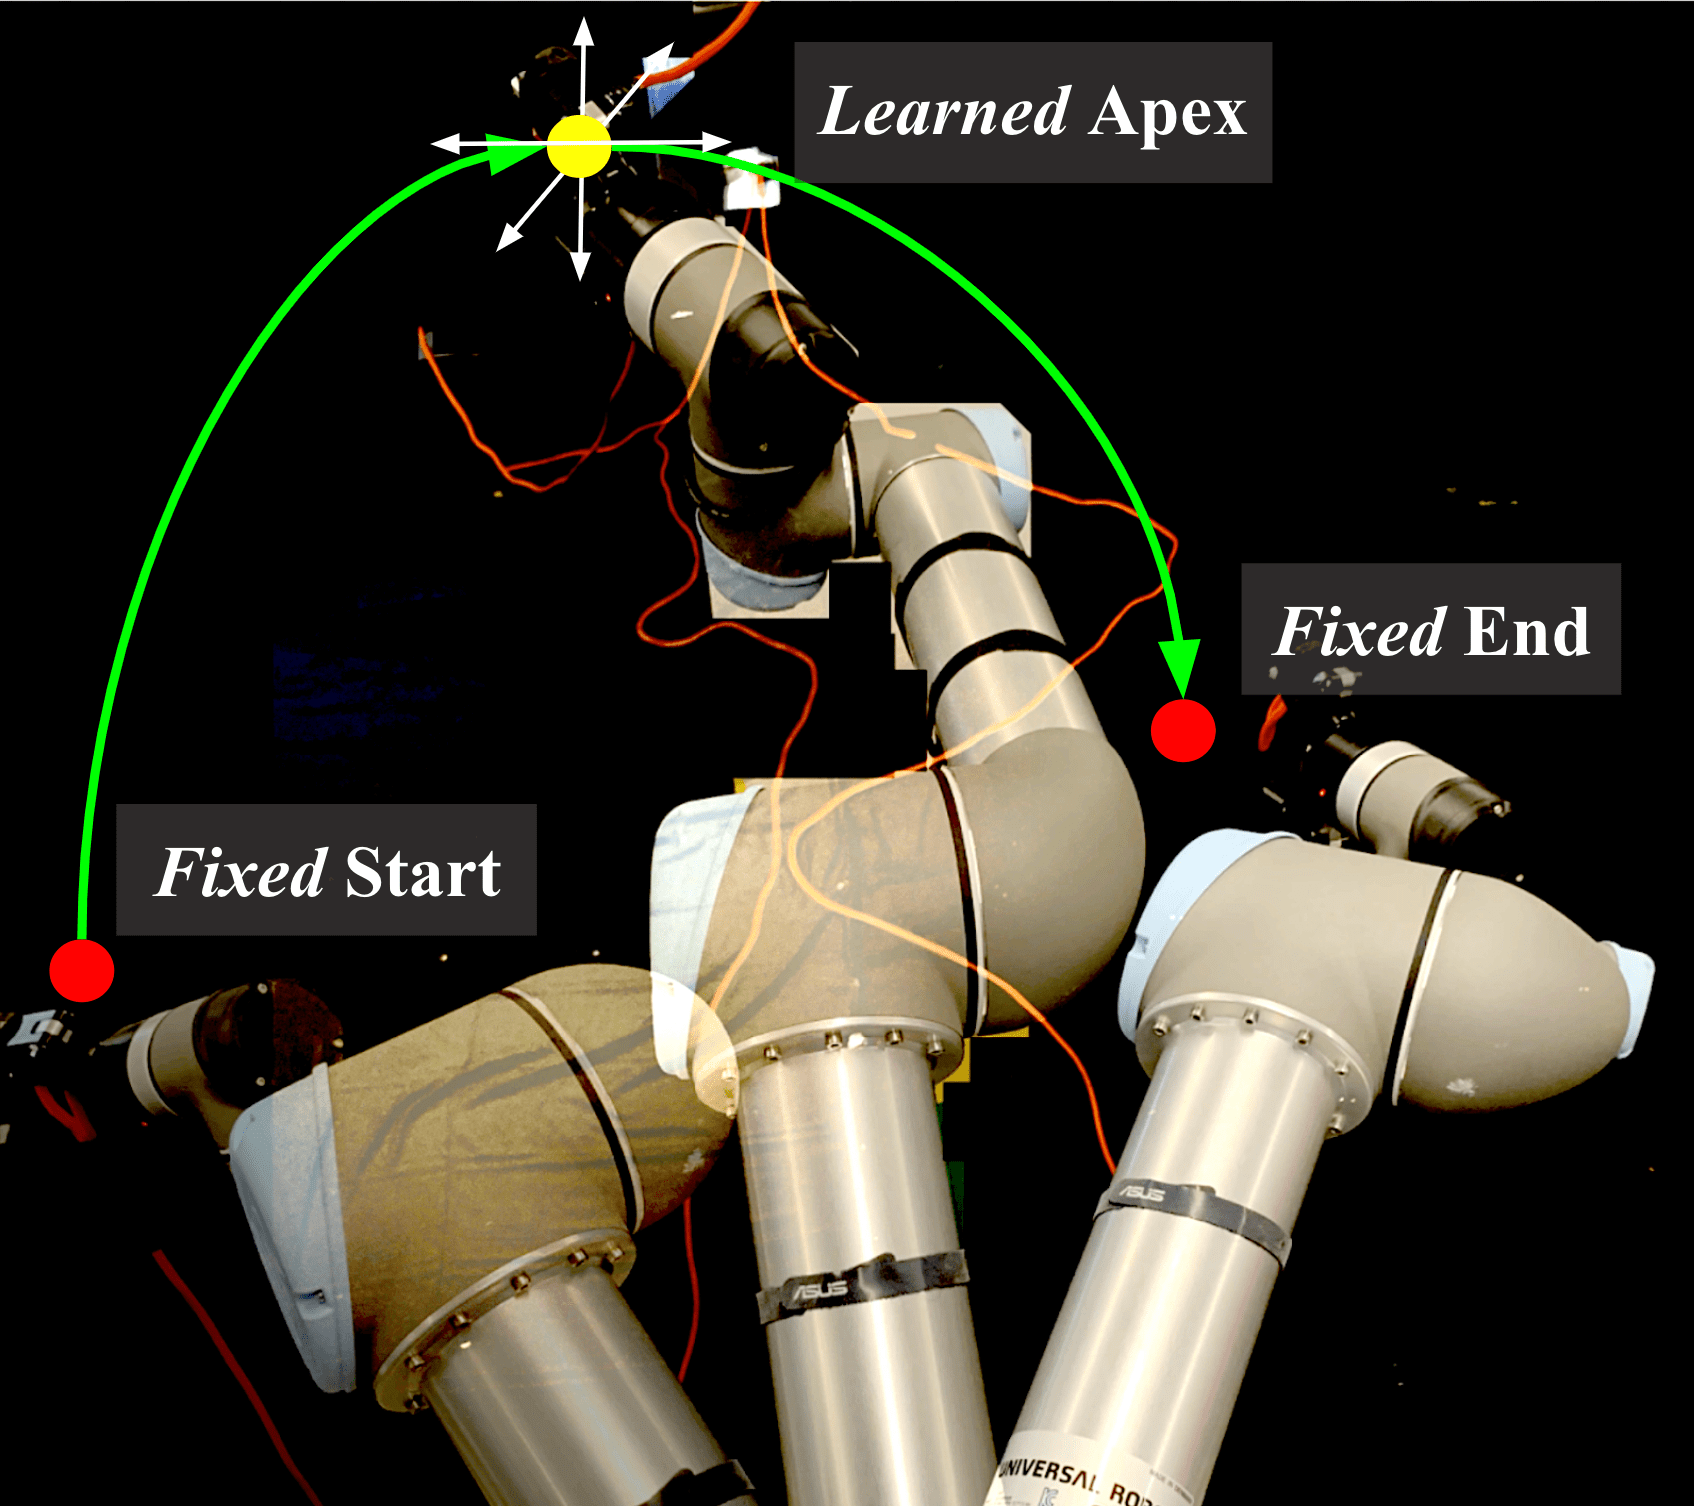
\includegraphics[width=\linewidth]{figures/3point.png}
%     \caption{Using three points in a curve to control the trajectory of the cable. The start and end points are fixed using the arm configurations. We change the trajectory by varying the apex configuration.}
%     %\vspace*{-10pt}
%     \label{fig:3point}
% \end{figure}


INDy uses a trajectory generation function $f_{\mathcal{A}_i} : \mathbb{R}^3 \rightarrow \mathcal{A}$ to reduce the output dimension of the neural network, % trained in Sec.~\ref{sec:deep_alg},
while still being able to achieve a high success rate on tasks.  In initial experiments, we observed that for the trajectory to be dynamically feasible, the trajectory generation must also limit and minimize jerk.  Otherwise, acceleration changes would often be too fast for the manipulator arm to follow while burdened by the inertia of the cable.

We propose a function based on a quadratic program (QP) that has these features and empirically achieves high success rates in the 3 tasks.  %To generate a trajectory, 
%We formulate and solve a quadratic program (QP). 
We first discretize a trajectory to $H+1$ time steps, each with $h$ seconds apart.  At each time step $t \in \irange 0H$, the discretized trajectory has a configuration $\vec{q}_t$, and a configuration-space velocity $\vec{v}_t$ and acceleration $\vec{a}_t$.  With constraints in the QP, we enforce that the trajectory is kinematically and dynamically feasible, starts and ends at 2 fixed arm configurations, and reaches an apex configurations defined by the output of the learned policy.  The objective of the QP minimizes jerk.  To make the trajectory as fast as possible, in a manner similar to GOMP~\cite{GOMP}, we repeatedly reduce $H$ by 1 until the QP is infeasible, and use the shortest feasible trajectory.  The QP takes the following form:
\begin{small}
\begin{align*}
    \argmin_{(\vec{q},\vec{v},\vec{a})_{\irange 0H}} \; & \frac 1{2h} \sum_{t=0}^{H-1} (\vec{a}_{t+1} - \vec{a}_{t})^{\intercal} Q (\vec{a}_{t+1} - \vec{a}_{t}) \\
    \text{s.t.} \; & \vec{q}_0 \text{ is the start configuration} \\
    & \vec{q}_{\lfloor H/2 \rfloor} \text{ is the apex configuration} \\
    & \vec{q}_H \text{ is at the end configuration} \\
    & \vec{v}_0 = \vec{v}_{H} = \vec{0} \\
    & \vec{q}_{t+1} = \vec{q}_t + h \vec{v}_t + \tfrac 12 h^2 \vec{a}_t \quad \forall t \in \irange 0{H-1} \\
    & \vec{v}_{t+1} = \vec{v}_t + h \vec{a}_t \quad \forall t \in \irange 0{H-1} \\
    & \vec{q}_\mathrm{min} \le \vec{q}_t \le \vec{q}_\mathrm{max} \quad \forall t \in \irange 1{H-1} \\
    & \vec{v}_\mathrm{min} \le \vec{v}_t \le \vec{v}_\mathrm{max} \quad \forall t \in \irange 1{H-1} \\
    & \vec{a}_\mathrm{min} \le \vec{a}_t \le \vec{a}_\mathrm{max} \quad \forall t \in \irange 0{H-1} \\
    & h \vec{j}_\mathrm{min} \le \vec{a}_{t+1} - \vec{a}_t \le h\vec{j}_\mathrm{max} \quad \forall t \in \irange 0{H-1}.
\end{align*}
\vspace*{-15pt}
\end{small}

%As with DJGOMP~\cite{DJGOMP}, the QP minimizes the sum of squared jerks (changes in acceleration) experienced in the joint space. 
%In physical experiments, minimizing and limiting the jerk was necessary to prevent automated E-stops due to physical motions deviating from planned high-jerk trajectories.  
The $Q$ matrix is a diagonal matrix that adjusts the relative weight of each joint.  The QP constraints, in order, fix the start, midpoint, and end configurations ($\vec{q}_0$, $\vec{q}_{\lfloor H/2 \rfloor}$, $\vec{q}_{H}$); fix the start and end velocity ($\vec{v}_0$, $\vec{v}_{H}$) to zero; enforce configuration and velocity dynamics between time steps ($\vec{q}_{t+1}$, $\vec{v}_{t+1}$); keep the joints within the specified limits of configuration ($\vec{q}_\mathrm{min}$, $\vec{q}_\mathrm{max}$), velocity ($\vec{v}_\mathrm{min}$, $\vec{v}_\mathrm{max}$), acceleration ($\vec{a}_\mathrm{min}$, $\vec{a}_\mathrm{max}$), and jerk ($\vec{j}_\mathrm{min}$, $\vec{j}_\mathrm{max}$).
%In addition, to minimize the trajectory time like GOMP, after solving the QP, we shrink the $H$ by $1$ and repeat the process until the QP is no longer solvable due to constraint violations.
Unlike GOMP, we do not consider obstacle avoidance in the trajectory generation, and instead ensure that there are no obstacles in the path of the arm to avoid.  In practice, we fix $h$ to be an integer multiple of the robot's control frequency, and the initial value of $H$ to be sufficiently large such that there is always a solution.

The input to the trajectory function constrains the midpoint configuration of the trajectory.  As most trajectories lift then lower the end effector through the midpoint, the input is often the apex of the motion.  With the UR5 robot, we observe that varying the first 3 joints (base, shoulder, elbow) moves the end-effector's location in $(x,y,z)$.  The base joint rotates left and right, while the shoulder and elbow joints lift and extend.  We thus use these 3 joints to define the midpoint, while having the remaining joint configurations depend linearly on the first three.
We make this function a task-specific function by constraining the start and end configurations to depend on the task.  For example, for the left-to-right vaulting task, we set the start configuration to be down and left, and the end configuration to be down and right.

\section{Simulatior}
\label{sec:sim2real}

We use simulation to experiment with training algorithms, and to find a feasible base action $a_\beta$ to bootstrap the data collection process in the real world.  Using simulation enables fast prototyping to efficiently assess qualitative and quantitative behavior of multiple base actions, but can suffer from a sim-to-real gap, motivating research teams to collect data from running robots in the real world~\cite{gupta2018,folding_fabric_fcn_2020}. Similarly, we collect data by running a physical UR5 robot, but use simulation as a means to obtain a functional action that can be improved upon when collecting data.

To model cables in simulation, we use a Featherstone~\cite{featherstone1984robot} rigid-body simulator from BulletPhysics via Blender~\cite{blender}. Cables consist of a series of small capsule links connected by spring and torsional forces. %spring constants, torsional stiffness, and damping coefficients that make the simulated cable behave physically similar to power cords we use in physical experiments. 
We tune the spring and torsional coefficients by decreasing bending resistance and stopping before the cable noticeably behaves like individual capsules rather than a cable, and increasing twist resistance until excessive torsion causes the capsules to separate.
%We use a 4:1 scale between simulation and real, because when the radius of the simulated cable is below 10 cm, the collision effects between capsules disconnect the cable.
%Specifically, in Blender, we use a torsional stiffness value of 1, a twist damping value of 0.9, a spring stiffness value of 40, and a spring damping value of 0.5.

When finding a feasible $a_\beta$ to transfer to real, we only simulate vaulting. The obstacle height, radius, and location are randomized for each trial, along with the initial cable state. We use 10 different obstacle and initial cable settings in simulation, and select the input apex point with highest success rate out of 60 random points. Then, we take this apex point directly to physical experiments as the base action $a_\beta$ to collect data, as the physical UR5 exhibits similar behavior to that in simulation after applying the predefined configurations from simulation, as seen in Fig.~\ref{fig:sim_to_real}.

% We use Blender~\cite{blender,priya_2020,descriptors_fabrics_2020}, as its keyframe feature allows us to specify robot configurations at certain animation frames, with the robot motion between keyframes being automatically interpolated. 

%Additionally, Blender has an easy to use Python API, and its built-in rendering engine Eevee supports ray-tracing, making rendering fast on GPUs.
% because it has previously worked reasonably well for manipulating 1D~\cite{priya_2020} and 2D structures~\cite{descriptors_fabrics_2020}.

% Using this setup, we compare the three-point arc model with different models. First, we tried regressing both apex point location and velocity explicitly, and found that regressing velocity did not improve the success rate of the vaulting task. We have also tried interpolating a straight-line motion between the points without making it arcing and found that the discontinuity in the middle causes the robot to come to a complete stop at the apex, thus reducing the energy stored for the cable to move fast enough.
